\documentclass[tikz,border=5pt]{standalone}

\begin{document}
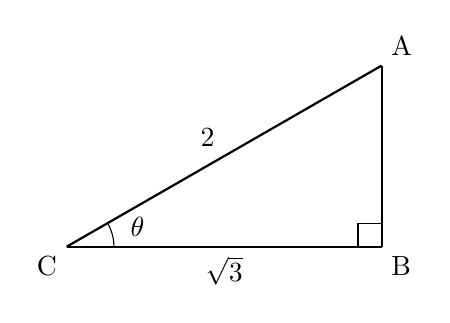
\begin{tikzpicture}

% Define coordinates for the triangle vertices
\coordinate (C) at (0,0);
\coordinate (B) at (4,0);
\coordinate (A) at (4,2.3);

% Draw the triangle sides
% Side CB (base)
\draw[thick] (C) -- (B);

% Side BA (vertical side)
\draw[thick] (B) -- (A);

% Side CA (hypotenuse)
\draw[thick] (C) -- (A);

% Draw right angle symbol at B
\draw (3.7,0) -- (3.7,0.3) -- (4,0.3);

% Draw angle arc for theta at C
\draw (0.6,0) arc (0:30:0.6);

% Label for angle theta at C
\node at (0.9,0.25) {$\theta$};

% Label for point A
\node[above right] at (A) {A};

% Label for point B
\node[below right] at (B) {B};

% Label for point C
\node[below left] at (C) {C};

% Label for hypotenuse CA (length 2)
\node[above left] at (2,1.15) {2};

% Label for base CB (length sqrt(3))
\node[below] at (2,0) {$\sqrt{3}$};

\end{tikzpicture}
\end{document}